\section{Boolean Algebra}
\subsection{An introduction to Boolean Algebra}

\textbf{Boolean Algebra} is a set of rules/operations for working with variables whose values are either 0 or 1.
It corresponds highly to propositional logic.

\textbf{Boolean Multiplication}, denoted by $\cdot$.
\begin{align*}
  \text{Boolean } & \cdot & \text{Logic }           & \land      \\
  0 \cdot 0       & = 0   & \text{F} \land \text{F} & = \text{F} \\
  0 \cdot 1       & = 0   & \text{F} \land \text{T} & = \text{F} \\
  1 \cdot 0       & = 0   & \text{T} \land \text{F} & = \text{F} \\
  1 \cdot 1       & = 1   & \text{T} \land \text{T} & = \text{T}
\end{align*}

\textbf{Boolean Addition}, denoted by $+$.
\begin{align*}
  \text{Boolean } & \cdot & \text{Logic }          & \lor       \\
  0 + 0           & = 0   & \text{F} \lor \text{F} & = \text{F} \\
  0 + 1           & = 1   & \text{F} \lor \text{T} & = \text{T} \\
  1 + 0           & = 1   & \text{T} \lor \text{F} & = \text{T} \\
  1 + 1           & = 1   & \text{T} \lor \text{T} & = \text{T} \\
\end{align*}

\textbf{Boolean Complement}, denoted by $\bar{ }$.
\begin{align*}
  \text{Boolean } & \bar{ } & \text{Logic }  & \lnot      \\
  \bar{0}         & = 1     & \lnot \text{F} & = \text{T} \\
  \bar{1}         & = 0     & \lnot \text{T} & = \text{F} \\
\end{align*}

\begin{center}
  \begin{circuitikz}
    \draw (0,0) to[battery] (0,2)
    to[switch, l=$x$] (2,2)
    to[switch, l=$y$] (4,2)
    to[lamp] (4,0) -- (0,0);
    \draw (2,-1) node[] {Shannon Circuit (AND $\cdot$)};
  \end{circuitikz}
  \qquad
  \begin{circuitikz}
    \draw (0,0) to[battery] (0,2) -- (1,2) -- (1,1.5)
    to[switch, l=$x$] (3,1.5) -- (3,2) -- (4,2) to[lamp] (4,0) -- (0,0)
    (1,2) -- (1,2.5)
    to[switch, l=$y$] (3,2.5) -- (3,2);
    \draw (2,-1) node[] {Switching Circuit (OR $+$)};
  \end{circuitikz}
\end{center}

Variables that can have a value of either $1$ or $0$ are called \textbf{Boolean Variables}.
Boolean expressions are made of boolean variables. There are also common shorthand ways of notating operations.
\begin{align*}
  x \cdot y + 1 \cdot \bar{z} & = xy + \bar{z}        \\
  x + z + \overline{0 + y}    & = x + z \cdot \bar{y}
\end{align*}

\begin{center}
  \begin{tabular}{r|c|c}
    \textbf{Law Name} & $+$ OR                                               & $\cdot$ AND                                          \\
    \hline
    Idempotent        & $x + x = x$                                          & $x \cdot x = x$                                      \\
    Associative       & $(x + y) + z = x + (y + z)$                          & $(x \cdot y) \cdot z = x \cdot (y \cdot z)$          \\
    Commutative       & $x + y = y + x$                                      & $x \cdot y = y \cdot x$                              \\
    Distributive      & $x + (y \cdot z) = (x + y) \cdot (x + z)$            & $x \cdot (y + z) = (x \cdot y) + (x \cdot z)$        \\
    Identity          & $x + 0 = x$                                          & $x \cdot 1 = x$                                      \\
    Domination        & $x + 1 = 1$                                          & $x \cdot 0 = 0$                                      \\
    Double Complement & $\overline{\overline{x}} = x$                                                                               \\
    Complement        & $x + \overline{x} =$ 1                               & $x \cdot \overline{x} =$ 0                           \\
    DeMorgan          & $\overline{x + y} = \overline{x} \cdot \overline{y}$ & $\overline{x \cdot y} = \overline{x} + \overline{y}$ \\
    Absorption        & $x + (x \cdot y) = x$                                & $x \cdot (x + y) = x$
  \end{tabular}
\end{center}

\subsection{Boolean functions}

A \textbf{boolean function} is a function which maps $B^k \rightarrow B$,
where $B = \{0,1\}$. For example, consider $f:B^3 \rightarrow B$

\begin{center}
  \begin{tabular}{ccc|c}
    $x$ & $y$ & $z$ & $f(x, y, z)$ \\
    \hline
    0   & 0   & 0   & 0            \\
    0   & 0   & 1   & 0            \\
    0   & 1   & 0   & 0            \\
    0   & 1   & 1   & 1            \\
    1   & 0   & 0   & 1            \\
    1   & 0   & 1   & 1            \\
    1   & 1   & 0   & 0            \\
    1   & 1   & 1   & 1
  \end{tabular}
  \qquad
  \begin{tabular}{ccc|cc}
    $x$ & $y$ & $z$ & $f(x, y, z)$                     \\
    \hline
    0   & 0   & 0   & 0            &                   \\
    0   & 0   & 1   & 0            &                   \\
    0   & 1   & 0   & 0            &                   \\
    0   & 1   & 1   & 1            & $\bar{x}yz$       \\
    1   & 0   & 0   & 1            & $x\bar{y}\bar{z}$ \\
    1   & 0   & 1   & 1            & $x\bar{y}z$       \\
    1   & 1   & 0   & 0            &                   \\
    1   & 1   & 1   & 1            & $xyz$
  \end{tabular}
\end{center}
This function is equivalent to $f(x,y,z) = x \overline{y} + yz$.
This can be determined using the boolean table and a strategy of combining the cases.
\begin{align*}
  f(x,y,z) & = \bar{x}yz + x\bar{y}\bar{z} + x\bar{y}z + xyz \\
           & = y(\bar{x}z + xz) + \bar{y}(x\bar{z} + xz)     \\
           & = y(z \cdot 1) + \bar{y}(x \cdot 1)             \\
           & = yz + \bar{y}x = \bar{y}x + yz                 \\
           & = x\bar{y} + yz
\end{align*}

A \textbf{literal} is a boolean variable or the complement of a boolean variable,
for example $x$ or $\bar{x}$. In a boolean function whose input variables are
$v_1, v_2, \ldots, v_k$, a \textit{mini-term} is a product of literals
$u_1, u_2, \ldots, u_k$, such that $u_j$ is either $v_j$ or $\overline{v_j}$

\subsection{Disjunctive and conjunctive normal form}

A boolean expression that is the sum of literals is said to be in \textit{disjunctive normal form},
\textbf{DNF}. It has the following form:
\[
  c_1 + c_2 + \cdots + c_m, \text{ where $c_j$ for $j \in \{1,\ldots,m\}$ is a product of literals.}
\]
For example, $\bar{x}y\bar{z} + xy + w + y\bar{z}w$. The complement only applies to a single variable and
\underline{no} addition within a term.

A boolean expression that is the product of sums of literals is said to be in \textit{conjunctive normal form},
\textbf{CNF}. It has the following form:
\[
  d_1 + d_2 + \cdots + d_m, \text{ where $d_j$ for $j \in \{1,\ldots,m\}$ is a sum of literals.} \\
\]
Each $d_j$ is called a clause, and complements are only applied to a single variable.
Additionally, there is no multiplication within variables.
An example is $(\bar{x} + y + z)(x + \bar{y})(w)(y + \bar{z} + w)$.

\subsection{Functional completeness}

A set of operators is functionally complete if any boolean function can be expressed using only operations from the set.
Two expressions can be added using only multiplication and complement.
\[
  x + y = \overline{\bar{x} \bar{y}} \text{ DeMorgan's Law}
\]
DeMorgan's Law can be extended to more than two boolean variables:
\[
  x + y + w + z = \overline{\bar{x} \bar{y} \bar{w} \bar{z}}
\]
The same can be said about the addition variant of the law:
\begin{align*}
  xy   & = \overline{\bar{x} + \bar{y}}                     \\
  xywz & = \overline{\bar{x} + \bar{y} + \bar{w} + \bar{z}}
\end{align*}

The \textbf{NAND} operation, $\uparrow$, and the \textbf{NOR} operation, $\downarrow$.
\begin{center}
  \begin{tabular}{cc|cc}
    $x$ & $y$ & $x \uparrow y$ & $x \downarrow y$ \\
    \hline
    0   & 0   & 1              & 1                \\
    0   & 1   & 1              & 0                \\
    1   & 0   & 1              & 0                \\
    1   & 1   & 0              & 0
  \end{tabular}
\end{center}

$\{\text{NAND}\}$ is functionally complete, it can create the complement,
from which all other possible gates can be created.
\begin{center}
  \begin{tabular}{c|c}
    $x$ & $x \uparrow x$ \\
    \hline
    0   & 1              \\
    1   & 0
  \end{tabular}
\end{center}
From the complement, AND can be created, and \{AND, COMPLEMENT\} has already been proven to be functionally complete.
\[
  xy = \overline{x \uparrow y} = (x \uparrow y) \uparrow (x \uparrow y)
\]

\subsection{Boolean satisfiability}

The \textbf{Boolean Satisfiability problem}, called the \textit{SAT} for short,
takes the boolean expression as an input and asks whether it is possible to set the values of the variables
so that the expression evaluates to 1.
\begin{align*}
  \text{If } & \exists x \exists y \ldots B(x, y, \ldots), \text{ then the expression is \textbf{satisfiable}}         \\
  \text{If } & \forall x \forall y \ldots \lnot B(x, y, \ldots), \text{ then the expression is \textbf{unsatisfiable}} \\
\end{align*}
Expressions in DNF form are very easy to determine satisfiability.
If there is \underline{any} term which does \textit{not} contain a variable and its complement,
it is satisfiable. For example,
\[
  x\bar{y}z\bar{x} + \overbrace{\bar{w}xy\bar{z}}^\text{no self-complements} + \bar{w}xw\bar{x} + xy\bar{z}z
\]
The above equation \textit{is} satisfiable because there is a term which does not contain a self-complement.

\subsection{Gates and circuits}

Circuits are built from electrical devices called \textbf{gates}.
\begin{center}
  \textbf{AND}:
  \begin{circuitikz}
    \draw (0,0) node[and port] (AND){}
    (AND.in 1) node[anchor=east] {$x$}
    (AND.in 2) node[anchor=east] {$y$}
    (AND.out) node[anchor=west] {$xy$};
  \end{circuitikz}
  \quad
  \textbf{OR}:
  \begin{circuitikz}
    \draw (0,0) node[or port] (OR){}
    (OR.in 1) node[anchor=east] {$x$}
    (OR.in 2) node[anchor=east] {$y$}
    (OR.out) node[anchor=west] {$x+y$};
  \end{circuitikz}
  \quad
  \textbf{NOT/INVERTER}:
  \begin{circuitikz}
    \draw (0,0) node[not port] (NOT){}
    (NOT.in) node[anchor=east] {$x$}
    (NOT.out) node[anchor=west] {$\bar{x}$};
  \end{circuitikz}
\end{center}

The boolean function $f(x_1,x_2): (f(x_1,x_2) \cdot x_1) + x_2$. Yes, circuits can contain recursion.
\begin{center}
  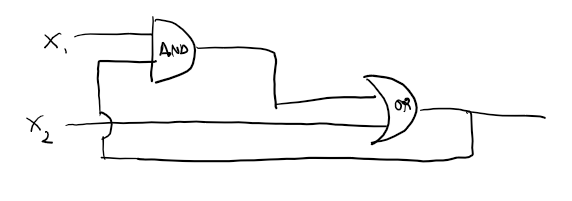
\includegraphics[width=.6\linewidth]{resources/recursive.png}
\end{center}

Boolean expressions can also be constructed by following the logic or a circuit.
\begin{center}
  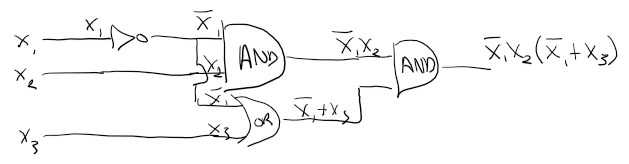
\includegraphics[width=.6\linewidth]{resources/construction_from_circuit.png}
\end{center}
\[
  f(x_1,x_2,x_3) = \bar{x}_1 x_2 (\bar{x}_1 + x_3)
\]

An example of constructing a circuit from a boolean expression, $f(x,y,z):(x+y)(\bar{z}+\bar{y})$
\begin{center}
  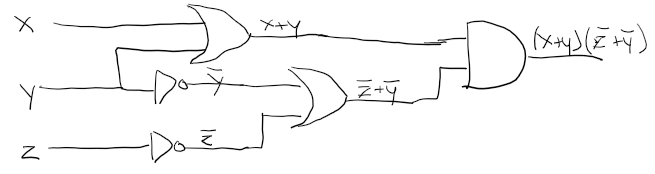
\includegraphics[width=.6\linewidth]{resources/construction_from_function.png}
\end{center}

\subsubsection{Designing Circuits}

\begin{enumerate}
  \item Build an input/output table with the desired output for every combination of input
  \item Construct a boolean expression that computes the same function as the function specified in the input/output table
  \item Construct a digital circuit that realizes the boolean expression
\end{enumerate}

I/O for sum of two bits, $x,y$
\begin{center}
  \begin{tabular}{cccc}
    x & y & m & l \\
    \hline
    0 & 0 & 0 & 0 \\
    1 & 0 & 0 & 1 \\
    0 & 1 & 0 & 1 \\
    1 & 1 & 1 & 0 \\
  \end{tabular}
\end{center}
\begin{align*}
  m & = xy                  & \text{most significant bit}  \\
  l & = x\bar{y} + \bar{x}y & \text{least significant bit}
\end{align*}
\begin{center}
  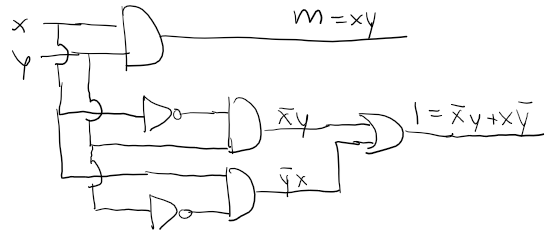
\includegraphics[width=.6\linewidth]{resources/sum_of_two_bits.png}
\end{center}
\begin{center}
  *\textit{this method does not necessarily give the most \underline{efficient} circuit}.
\end{center}
Circuits with fewer gates cost less to manufacture. Here is a simplified circuit to add two bits:
\begin{center}
  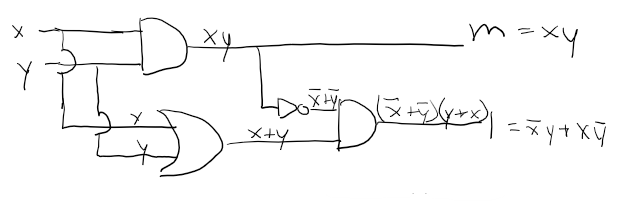
\includegraphics[width=.6\linewidth]{resources/better_sum_of_two_bits.png}
\end{center}

Here is another example with boolean logic for light switches:
\begin{center}
  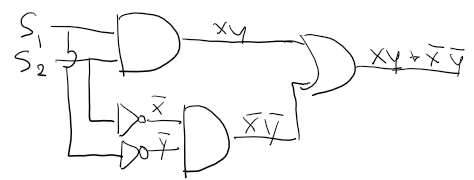
\includegraphics[width=.6\linewidth]{resources/switches.png}
\end{center}